\documentclass[a4paper,14pt]{extreport}

\usepackage[T2A]{fontenc}
\usepackage[utf8]{inputenc}
\usepackage[ukrainian]{babel}

\usepackage{lastpage}
\usepackage{graphicx}
\usepackage{url}
\usepackage{listings}
\lstset{frame=single,basicstyle=\ttfamily\scriptsize,extendedchars=\true}

\usepackage{amssymb}

\newtheorem{lemma}{Лема}
\newtheorem{theorem}{Теорема}
\newtheorem{proposition}{Твердження}

\usepackage{multirow}
\usepackage{array}

% maybe unused
\usepackage{longtable}

\usepackage{zvit}

\usepackage[unicode]{hyperref}
\hypersetup{colorlinks=false}

% for literature
\usepackage{datetime}
\renewcommand{\dateseparator}{.}
\newcommand{\todayiso}{01.09.2024}

\usepackage{bibspacing-report}
\setlength{\bibspacing}{\baselineskip}


% --- Zvit Settings -----

\NirOrgLongName{Львівський національний університет ім. І.Я. Франка

12345, Офіційна адреса

тел. (044) 123-45-67} %% 

\NirBoss{Директор Інституту Назва \newline
 НАН України \newline
академік НАН України}{ПІБ директора} 
\NirManager{доктор фізико-математичних наук, професор}{ПІБ Керівника} 


\NirYear{2024}
\NirTown{м. Львів,} 
 
\NirDate{~~~ 2024 р.}


\NirUdk{517.958:539.37}
\NirGosNo{№ держреєстрації 0000U000001}

\NirStage{не використовується}{заключний}{}



\begin{document}

\usefont{T2A}{ftm}{m}{n} 

% Add C. to start of contents
\cftaddtitleline{toc}{part}{}{С.}

\frontmatter 

% Title page
\thispagestyle{empty}

УДК \quad 000.000.00

 \begin{centering}
  \linespread{1.1}
  \vspace{2em}

{Національна академія наук України

Назва інституту}

  \vspace{5em}

ПРІЗВИЩЕ Ім'я По-батькові

  \vspace{2em}

Розвиток архітектури та методів автоматичної компіляції дисертацій

у середовищі Latex

  \vspace{5em}


Дисертація 

на здобуття наукового ступеня кандидата технічних наук

за спеціальністю 05.13.05 -- комп'ютерні системи та компоненти


  \vspace{2em}

\textit{Науковий керівник}

доктор фізико-математичних наук

професор

ПІБ Керівника

\vspace{11em}

  Київ -- 2018

 \end{centering}
\begin{flushright}
 На правах рукопису
\end{flushright} 
% End of Titlepage

\tableofcontents

\chapter{ВСТУП}

%Hidden cite for correct bibliography ordering
\nocite{bahvalov-et-al,benerdge-et-al} 

\textbf{Актуальність теми.}

Традиційне хірургічне втручання або відкрита хірургія характеризується відносно великим розтином м'яких тканин. Для 
доступу до органу над яким хірург має провести маніпуляцію також треба зупинити кровотечу спричинену розтином. Ці дії 
проводяться в умовах стерильності, які серйозно обмежують кількість рухів, які виконує лікар. Це зменшує комфорт 
проведення операційного втручання.

З іншої сторони великий розтин дозволяє отримати широкий кут огляду місця провення хірургічної операції. Проте така 
зручність супроводжується суттєвими недоліками:
\begin{itemize}
  \item Збільшення ймовірності інфекції.
  \item Суттєві больові відчуття у пацієнта\textbackslashпацієнтки після операції.
  \item Довший період реабілітації від хірургічного втручанння.
  \item Великий шрам у місці розтину.
\end{itemize}

Головним фактором вищезгаданих недоліків є великий розтин у м'яких тканинах. Тому були створені нові методи 
малоінвазивної хірургії. Суттєва різниця полягає у розмірі отвору через який вводяться хірургічні інструменти. 
Зокрема у лапароскопічній операції, яка є одним із підвидів малоінвазивної хірургії, через отвори утворений в результаті 
проколу м'яких тканин вводяться інструменти. Серед них є ендоскоп, який виводить зображення на монітор і освітлює місце 
проведення операції.

\begin{figure}[h!]
  \centering
  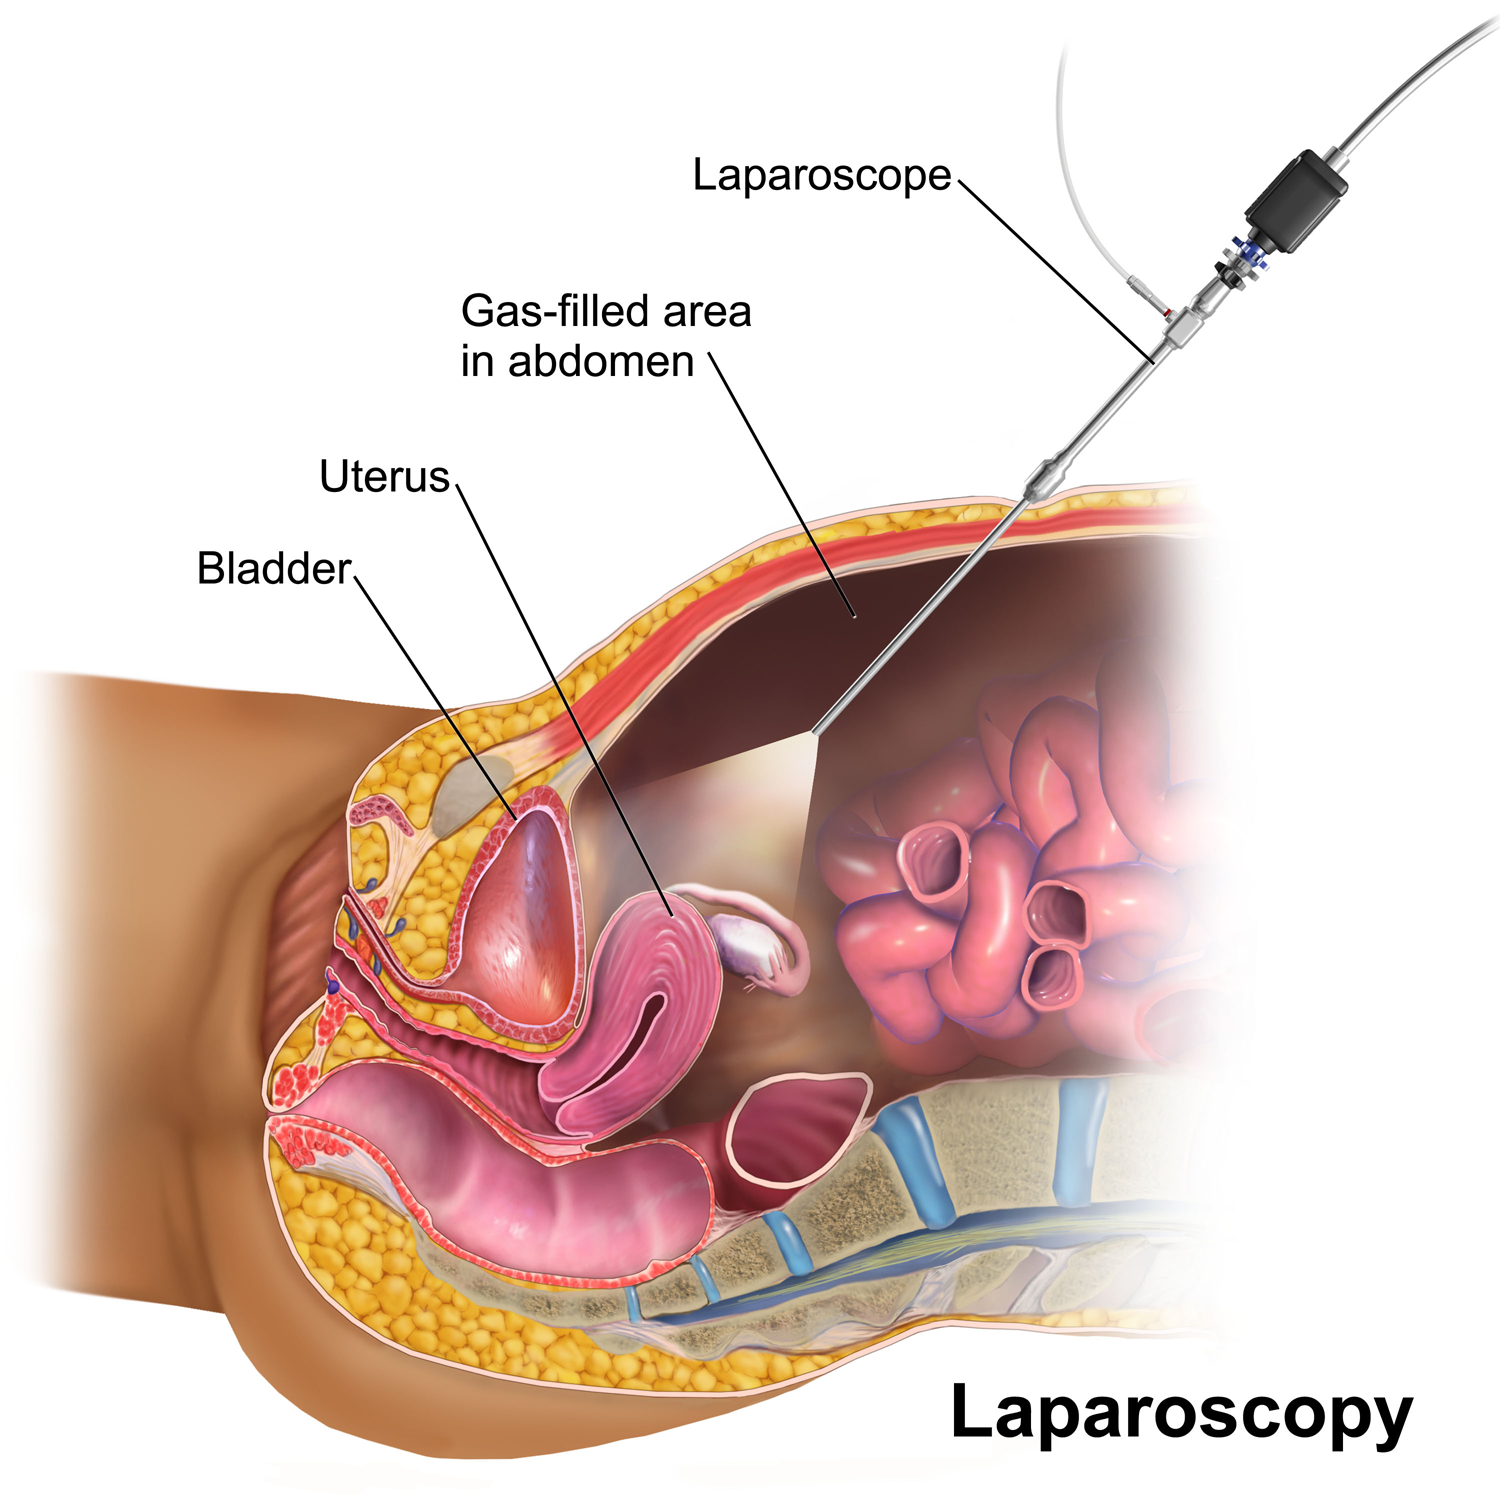
\includegraphics[width=0.4\linewidth]{images/intro_laparoscopy.png}
  \caption{Лапароскопія.}
  \label{fig:intro_laparoscopy}
\end{figure}

Лапароскопічні операції (рис. \ref{fig:intro_laparoscopy}) є кроком вперед проте мають ряд недоліків
\begin{itemize}
  \item Збільшення ймовірності інфекції.
  \item Суттєві больові відчуття у пацієнта\textbackslashпацієнтки після операції.
  \item Довший період реабілітації від хірургічного втручанння.
  \item Великий шрам у місці розтину.
\end{itemize}

Малоінвазивна робото хірургія. 


Більшість елементів сучасного приводу, конструкцій чи побутові речі виготовлені із гетерогенного матеріалу, зокрема із композиційного матеріалу або композиту. Тому виникає потреба у розробці методів, які б дозволяли розраховувати напружено-деформований стан, а також температуру.

Широко вживаними протягом кількох десятиріч методом розв'язування задач такого класу є проекційно-сітковий метод або метод скінчених елементів (МСЕ). Завдяки таким властивостям як розрідженість і симетричність матриць для класу задач у локально-неоднорідних тілах, різні варіанти МСЕ набули популярності.

Із МСЕ цілком успішно може конкурувати, а іноді бути ефективнішим,
велике сімейство методів граничних елементів
(МГЕ) \cite{benerdge-et-al} {[}4{]}{[}6{]}{[}7{]}{[}9{]}{[}12{]}{[}16{]}, які базуються
на ідеях розроблених С.Г.Міхліном{[}19{]}, Н.І.Мусхелішвілі{[}20{]},
В.Д.Купрадзе{[}17{]} та інші. Ці обставині особливо сприяють такі
переваги, як зменшення на одиницю геометричної розмірності задачі,
простота розв'язування для безмежних областей, можливість обчислювати у
лінійних задачах значення шуканих величин у довільній точці без нової
апроксимації, простота дискретизації.

У свою чергу серед класу МГЕ можна виділити такі методи як комплексний
метод граничних елементів (КМГЕ) і метод при граничних елементів (МПГЕ).
На відміну від КМГЕ, який є видозміненим варіантом класичного МГЕ, МПГЕ
базується на більш радикальніших ідеях. У порівнянні із МГЕ, МПГЕ
простіший для реалізації, проте у більшості випадків дає точніші
результати при тих самих затратах обчислювальних ресурсів.

Наукове завдання дисертаційної роботи -- розробка ефективного методу для
розв'язування задач термопружності у композитах є актуальною проблемою.

\textbf{Зв'язок роботи з науковими програмами, планами та
темами.} Робота виконувалась на кафедрі програмування львівського
національного університету імені Івана Франка, а також у інституті
прикладних проблем механіки і математики імені Ярослава Підстригача НАН
України, відділ термомеханіки в рамках держбюджетної теми ``Розробка
аналітико-чисельних методів дослідження напруженого стану неоднорідних
тіл з тепловими та залишковими деформаціями і дефектами структури''.
(!!! Номер теми !!!)

\textbf{Мета роботи та задачі дослідження.} Метою роботи є:

\begin{itemize}
\item
  побудова нових методів розв'язування задач термопружності у композитах
\item
  дослідження ефективності нових методів
\item
  порівняння швидкості збіжності і використання ресурсів із відомими
  методами
\end{itemize}

\emph{Об'єктом} дослідження є композити.

\emph{Предметом} дослідження є нові методи розв'язування задач
термопружності для композитів.

\emph{Методи дослідження.} Для розв'язування поставлених задач
використовується метод поєднання граничних і скінчених елементів.

\textbf{Наукова новизна одержаних результатів.} Наступні
результати отримані у роботі є новими:

\begin{enumerate}
\def\labelenumi{\arabic{enumi}.}
\item
  побудований метод на основі КМГЕ і МСЕ для розв'язування задачі
  теплопровідності у тілах із локальними неоднорідностями
\item
  для тіл із локальними неоднорідностями побудований метод на основі
  МПГЕ і МСЕ для розв'язування задач:

  \begin{enumerate}
  \def\labelenumii{\alph{enumii}.}
  \item
    пружності
  \item
    термопружності
  \end{enumerate}
\end{enumerate}

\textbf{Практичне значення отриманих результаті.} Отримані
результати дозволяють ефективніше розв'язувати актуальні проблеми, які
ставить перед нами народне господарство.

\textbf{Апробація результатів дисертації.} Основні результати
виконаних досліджень доповідалися та обговорювалися на:

\begin{enumerate}
\def\labelenumi{\arabic{enumi}.}
\item
  Восьмій Всеукраїнській науковій конференції (25-27 вересня 2001 р., м.
  Львів) ``Сучасні проблеми прикладної математики та інформатики'';
\item
  Дев'ятій Всеукраїнській науковій конференції (24-26 вересня 2002 р.,
  м. Львів) ``Сучасні проблеми прикладної математики та інформатики'';
\item
  Десятій Всеукраїнській науковій конференції (23-25 вересня 2003 р., м.
  Львів) ``Сучасні проблеми прикладної математики та інформатики'';
\item
  Одинадцятій Всеукраїнській науковій конференції (!!! 2004р., м. Львів)
  ``Сучасні проблеми прикладної математики та інформатики'';
\item
  Дванадцятій Всеукраїнській науковій конференції (4-6 жовтня 2005р., м.
  Львів) ``Сучасні проблеми прикладної математики та інформатики'';
\item
  Науковому семінарі ІППММ НАНУ імені Я.С.Підстригача, присвяченої
  пам'яті Є.Г.Грицька (22 квітня 2003 р., м. Львів);
\item
  Шостій Міжнародній науковій конференції (26-29 травня 2003 р., м.
  Львів) ``Математичні проблеми механіки неоднорідних структур'';
\item
  Семінар інституту прикладних проблем механіки та математики ім. Я.
  Підстригача
\end{enumerate}

У повному обсязі робота доповідалася на семінарі кафедри програмування
львівського національного університету імені Івана Франка.

\textbf{Публікації.} Результати досліджень висвітлені в 4 статтях
у журналах з переліку фахових видань ВАК України, в тому числі у
доповідях НАН України.

\textbf{Особистий внесок здобувача.} Всі результати дисертаційної
роботи отримано здобувачем самостійно.

\textbf{Структура та обсяг роботи.} Дисертація складається із
вступу і шести розділів основної частини, висновків, списку використаної
літератури із 37 найменувань.

У першому розділі описано підходи до розв'язування задач термопружності
і підхід, який був вибраний у даній роботи. Проаналізовано переваги і
недоліки кожного із запропонованих методів.

Другий розділ містить опис двох підходів для розв'язування задачі
теплопровідності. Перший підхід базується на ідеї предиктор-коректор, а
другий -- на рівняннях нев'язки у точках областей локальної
неоднорідності коефіцієнта теплопровідності.

Метод адитивного розчеплення оператора застосований для задачі пружності
для локально-неоднорідного тіла запропонований у третьому розділі. Даний
підхід був апробований для двох методів МГЕ і МПГЕ. Наведено порівняння
чисельних результатів для цих двох методів, а також порівняння методів
по інших критеріях, таких як простота реалізації, точність, діагональне
переважання матриць.

Четвертий розділ містить порівняльний аналіз МГЕ і МПГЕ при розв'язуванні задачі пружності у кусково-однорідному тілі. Наводяться рекомендації щодо застосування даних підходів для розв'язування задач такого класу.

У п'ятому розділі наведено підхід на основі МГЕ і МПГЕ для розв'язування
задачі термопружності у тілі із локально-неоднорідними властивостями
фізичних параметрів.

Програмне середовище Aspirant's Calculations Envinronment (ACE) було
створене для простого і зручного програмування запропонованих методів.
Структура даного середовища описана у шостому розділі. Також дано
рекомендації відносно використання даного середовища для програмування
подібних методів, яке вимагає невеликих зусиль спрямованих тільки на
побудову алгоритму, але не на організацію взаємодії між об'єктами.

\textbf{Усталені домовленості.} У цій праці кома перед індексом
означає похідну по змінній, яка відповідає цьому індексу, тобто
 ${f_{,j} = \partial}{f/\partial}x_{j}$, ${{f_{,ij} = \partial^{2}}{f/\partial}x_{i}\partial x_{j}}{}$,
при цьому викори­стовується німе сумування за індек­сами, які
повторюються.


\mainmatter %% turns on page numeration for pages below

\chapter{МЕТОДИКА ПОЄДНАННЯ ГРАНИЧНИХ І СКІНЧЕНИХ ЕЛЕМЕНТІВ}

%Hidden cite for correct bibliography ordering
\nocite{bahvalov-et-al,benerdge-et-al} 

\section{Огляд методів розв'язування задач термопружності у композитах}

Існують різні підходи, які найбільш часто використовують при дослідженні напружено-деформованого стану тіл.
Коротко зупинимось на деяких з них. З допомогою методу збурення форми
границі {[}\protect\hyperlink{anchor-15}{27}{]} на основі загальних
розв'язків задач теорії пружності для сфери, циліндра і еліпсоїда
обертання одержані наближені розв'язки задач для ізотропного середовища
з включеннями, гранична поверхня яких близька до вказаних. Головною
перевагою цього методу є те, що розв'язок задачі одержується в
замкнутому вигляді, а істотним недоліком те, що для побудови розв'язку
форма поверхні кусково-однорідного тіла і включень має вирішальне
значення. Тому клас задач, які розв'язуються цим методом, обмежений
тілами, граничні поверхні та поверхні розділу середовищ яких є
поверхнями другого порядку та близькими до них, зокрема, в
{[}\protect\hyperlink{anchor-16}{28}{]} розглянута для тривимірного
ізотропного пружного тіла з еліпсоїдальним включенням під дією
одновісного розтягу пружна задача, яка зведена до розв'язування системи
трьох інтегро-диференційних рівнянь відносно стрибків напружень і
переміщень на поверхнях включення, знайдено точний розв'язок цих рівнянь
і виписано формули для наближеного обчислення напружень у матриці і
включенні.

Однак при розв'язуванні багатьох практично важливих задач теорії
пружності потрібно розглядати тіла, поверхні контакту в яких мають
найрізноманітнішу форму. В зв'язку з цим широкого застосування набув
метод R-функцій {[}\protect\hyperlink{anchor-17}{29}{]}, який дає
можливість точно задовольняти граничні умови та умови спряження на
поверхнях контакту, але вимагає розвинутого спеціального математичного
та програмного забезпечення.

У багатьох роботах автори використовують деякі допущення про характер
контакту, зокрема в {[}\protect\hyperlink{anchor-18}{30}{]} розглянуто
задачі про контактну взаємодію двох скінченних стрингерів (накладок) з
різних пружних матеріалів із лінійно-деформованими основами (плоска
деформація) у вигляді пружної нескінченної смуги й анізотропної
півплощини в допущенні, що один із стрингерів перебуває в ідеальному
контакті з основою, а інший контактує з нею через тонкий шар клею.
Задачі зводяться до систем інтегро-алгебричних рівнянь другого роду. У
роботі {[}\protect\hyperlink{anchor-19}{31}{]} за допомогою аналітичних
комплекс­них потенціалів побудовано алгоритм розв'язування плоскої
задачі теорії пружності для трьохкомпонентної композиції, в якій границя
розділу матриці і включення моделюється пружним прошарком, а також дано
кількісну оцінку залежності узагальнених коефіцієнтів концентрації
напружень біля вершини криволі­нійного вирізу і абсолютно жосткого
включення від типу навантаження, пружних характеристик і ширини пружного
прошарку.

Оскільки аналітичний розв'язок багатьох практично важливих задач
(наприклад, для тіл з вирізами і неоднорідними включеннями) часто
утруднений, широкого використання набули числові методи, зокрема,
найбільш повно вивчені методи скінченних різниць
{[}\protect\hyperlink{anchor-20}{32}{]} та скінченних елементів. Вони
застосовуються здебільшого до плоских задач для розрахунку
напружено-деформованого стану пластин, оболонок, осесиметричних та
кусково-однорідних тіл.

Все більшої популярності при розв'язуванні задач набувають МГЕ
{[}\protect\hyperlink{anchor-2}{2}{]}, які ґрунтуються на ідеях,
розроблених С.Г.Міхліним, Н.І.Мусхелішвілі, В.Д.Купрадзе. Перевагами
методу граничних елементів (МГЕ), зокрема, є зниження на одиницю
розмірності задачі внаслідок дискретизації тільки граничної поверхні,
інтегральне зображення розв'язку є кращим, ніж числове диференціювання в
МСЕ, значно простіше досліджуються задачі для нескінчених областей.
Недоліком МГЕ є неможливість розгляду неперервно-неоднорідних тіл, а
також ускладнення алгоритму внаслідок обчислення сингулярних інтегралів.
Порівняння переваг різних методів привело до ідеї доцільності їх
поєднання і до створення на їх основі ефективних числово-аналітичних
методик, які дозволяють оптимізувати процес розв'язування {[}6{]}. У
роботі {[}\protect\hyperlink{anchor-21}{33}{]} побудовано об'єднаний
підхід МГЕ та МСЕ для розв'язання двовимірної статичної задачі теорії
пружності, що дозволяє звести вихідну задачу до послідовності розв'язків
підзадач у підобластях кожним із методів окремо, та розглянуто задачу
про плоску деформацію жорстко защемленого на одній із поверхонь шару під
рівномірно розподіленим навантеженням.

Одним з ефективних методів розрахунку напружень в кусково-однорідних
тілах є підхід, який ґрунтується на математичній постановці відповідних
узагальнених задач спряження, коли на основі частково вироджених
диференціальних рівнянь квазістатичної задачі термопружності для тіла з
чужорідними включеннями отримуються граничні інтегральні рівняння, єдині
для всієї розглядуваної області, які розв'язуються за допомогою прямого
МГЕ, при цьому враховуються умови ідеального та неідеального контакту
{[}\protect\hyperlink{anchor-22}{34},
\protect\hyperlink{anchor-23}{35}{]}.

МПГЕ {[}\protect\hyperlink{anchor-24}{14}{]}, який виник під впливом
методів граничних інтегральних рівнянь, проекційно-сіткових, занурення,
граничних і скінченних елементів та теорії синтезу математичних
алгоритмів, можна розглядати як один з варіантів методу джерела і
віднести його до непрямих методів досліджень, оскільки введені для
одержання розв'язку задачі невідомі не є фізичними змінними. У роботі
{[}\protect\hyperlink{anchor-25}{36},
\protect\hyperlink{anchor-26}{37}{]} зроблено порівняльний аналіз
теоретичних та обчислювальних особливостей МГЕ та МПГЕ для другої
основної задачі пружності та досліджено точність отриманих числових
результатів.

У даній роботі на основі підходів, запропонованих в
{[}\protect\hyperlink{anchor-2}{2}, \protect\hyperlink{anchor-19}{31},
\protect\hyperlink{anchor-24}{14}{]} для розв'язу­вання змішаної
статичної задачі теорії пружності неоднорідних тіл, змодельовано
напружено-деформований стан об'єктів та порів­няно точ­ність отриманих
МПГЕ і МГЕ розв'язків.

\section{Метод приграничних елементів}

TODO

\section{Суть методу поєднання граничних і приграничних елементів}

Одним із недоліків МГЕ є неможливість його застосування у тілах із
локальними неоднорідностями. Для розв'язання цієї проблеми був
запропонований підхід {[}\protect\hyperlink{anchor-5}{7}{]}. Основна
ідея даного підходу полягає у розчеплення оператора задачі на дві
частини, одна із них представляє оператор для однорідного тіла, для якої
МГЕ застосовний, а друга частина містить невідому функцій і
переміщується у праву частину рівняння. Ми отримуємо рівняння, яке за
своїм виглядом нагадує рівняння Пуасона, проте права частина містить
функцію залежну від шуканої функції. Для розв'язування даної проблеми
застосовуються різні підходи, а саме: а) метод пре диктор-коректор б)
метод нев'язок

У наступних розділах подані використання зазначених методик для задач
теплопровідності, пружності і термопружності у тілах із локальними
неоднорідностями.



\backmatter

% \chapter{ЗАГАЛЬНІ ВИСНОВКИ}

\chapter{ВИСНОВКИ}

За результатами виконання проекту можна зробити наступні висновки.

\begin{enumerate}
\item Результат.
\item Результат.
\end{enumerate}





\mainmatter

\clearpage
\addcontentsline{toc}{chapter}{ПЕРЕЛІК ПОСИЛАНЬ}
\bibliographystyle{plain}
\bibliography{literatura}

\appendix

%Fix Cyrillic letters in appendix numbering
\makeatletter
% Fix Title format
\gdef\thechapter{\@Asbuk\c@chapter}
\makeatother
\titleformat{\chapter}
  {\normalfont \centering}
  {ДОДАТОК~\Asbuk{chapter}~}{0pt}{}
\titlespacing{\chapter}{0cm}{0em}{3em}

% %\chapter{РЕАЛІЗАЦІЯ МОДУЛЯ ЗБОРУ СТАТИСТИКИ}
\label{app-module-for-statistics-gather}

Для відображення даних з черги задач СКЗ та виконання розрахунку статистики роботи кластера розроблений Perl-модуль системи портала кластерних обчислень. Цей модуль  виконує обробку вхідного текстового лог-файлу менеджера ресурсів SLURM, а на виході формує оброблені дані черги задач, відфільтрованих за певном критерієм та обчислює статистичні показники, розглянуті вище. Модуль працює в автономному режимі (запуск за запитом з консолі) та доданий до функціоналу порталу кластерних обчислень.

Perl-модуль використовує файл конфігурації підсистеми hydra порталу кластерних обчислень, розміщену в /opt/hydra/etc/hydra.conf. Конфігураційні дані відображені на рис.~\ref{fig:slurm.perl}.

\begin{figure}[!hb]
\begin{lstlisting}
##Job-log section
#Path for job-log file or pipe command "cmd|"
JOB_LOG_FILE="ssh n1000 cat /var/log/slurm.job.log|"
#Identifie usernamemes from uid's in job-log, can by "yes" or "no",
LOG_USER_IDENT="yes"
\end{lstlisting}
  \caption{Конфігурація Perl-модуля статистики роботи кластера}
 \label{fig:slurm.perl}
\end{figure}

Параметр \textbf{JOB\_LOG\_FILE} вказує шлях до вхідного лог-файла SLURM або є конвеєрною командою, якщо лог-файл знаходиться на іншому сервері. Параметр \textbf{LOG\_USER\_IDENT} вказує ідентифікувати чи ні імена користувачів по їхнім  UID. Керівний демон SLURM кластера СКІТ  slurmctld функціонує на сервері, який з метою безпеки не забезпечує аутентифікацію користувачів через LDAP. У наслідок чого slurmctld не може по UID користувача, що запустив задачу, визначити його імені. Через це в лог-файлі черги задач фігурують тільки UID користувачів, а ім'я ідентифікується як Unknown. Саме для таких випадків і потрібна ця опція. Perl-модуль  напряму з’єднується з LDAP-сервером, та отримує від нього необхідну інформацію. Параметри підключення беруться з файла адміністративної конфігурації підсистеми hydra порталу кластерних обчислень, розміщену у \textbf{/opt/hydra/etc/hydra-adm.conf}. Параметри налаштування роботи з LDAP-сервером відображені на рис.~\ref{fig:slurm.perl.conf}.

\begin{figure}[!hb]
\begin{lstlisting}
# User database management system LDAP,PASSWD
USERDB=LDAP
# LDAP Parameters
LDAP_HOST=10.0.0.254
#LDAP_SEARCH_BASE="dc=cluster,dc=icyb"
LDAP_SEARCH_BASE="ou=People,dc=cluster,dc=icyb"
LDAP_ADM_DN="cn=ldapadm,dc=cluster,dc=icyb"
LDAP_ADM_PASSWD="password"
\end{lstlisting}
  \caption{Конфігурація Perl-модуля статистики роботи кластера для роботи з базою LDAP}
 \label{fig:slurm.perl.conf}
\end{figure}

Додатково модуль виконує обрахунок тривалості кожної задачі за часом її запуску та завершення. Цей параметр використовується у розрахунках статистики, а також виводится у форматі ''дні -- години : хвилини : секунди'' при відображенні інформації з черги задач. Модуль може відфільтровувати чергу задач за наступними параметрами:

\begin{itemize}
\item початкова та кінцева дата, в межах року, що задають період, за яким відображатиметься інформація про завершені задачі;
\item ім’я користувача (у профілях користувачів порталу кластерних обчислень завжди виводиметься інформація, відфільтрована цим критерієм);
\item статус завершення задачі.
\end{itemize}

Особливістю ведення журналу задач системи SLURM є відсутність значення року у датах запуску та завершення задач, тому необхідно розділяти лог-файли за роками.

Приклад результуючого виводу стану завершених задач, придатного для відображення в табличному вигляді системою порталу кластерних обчислень, зображений на рис.~\ref{fig:job.log}.

\begin{figure}[!hb]
\begin{lstlisting}
22988 solo(15026) run.ompi run.ompi COMPLETED scit3 20000 11/02-13:29:45
      11/02-13:29:47 0-0:0:2 n3137 1 8
22799 ru(5005) part2 part2 COMPLETED scit3 20000 10/27-13:30:09
      11/02-14:10:55 6-0:40:46 n[3106-3112,3143] 8 64
22990 yershov(5599) btree btree FAILED scit3 120 11/02-14:10:56
      11/02-14:15:34 0-0:4:38  n[3106-3112,3143] 8 64
22991 vgor(1111) gms gms COMPLETED scit3 20000 11/02-14:15:36
      11/02-14:38:43 0-0:23:7 n[3106-3109] 4 32
22987 engraver(1255) D78h26_searchField D78h26_searchField
      CANCELLED scit3 300 11/02-12:43:48 11/02-15:43:04 0-2:59:16 n3119 1 8
22996 engraver(1255) vortexD78h26 vortexD78h26 CANCELLED scit3 600
      11/02-15:43:16 11/02-16:01:55 0-0:18:39 n3119 1 8
\end{lstlisting}
  \caption{Розпарсений вивід стану завершених задач}
 \label{fig:job.log}
\end{figure}

Розрахована статистика відображається як для окремого користувача, так і в загальному по кластеру. Системним адміністраторам порталу доступне відображення статистики за всіма користувачами одночасно. Приклад відображення статистики використання кластера за січень  поточного року зображено на рис.~\ref{fig:job.stat}.

\begin{figure}[!hb]
\begin{lstlisting}
# ./ic_get_jobstat -s -b 01/01 -e 02/01
USER:JobCount,JobRatio(%),CD,CA,F,NF,TO,AvgJobTime(min),Load(TotalTime(min)*NCPU),LoadRatio(%)
Chobal: 30      1.35%   27      2       0       0       1       1552    1477135 27.41%
akn:    61      2.75%   50      5       6       0       0       5       2463    0.05%
alex:   124     5.58%   90      10      15      0       9       0       463     0.01%
belous: 43      1.94%   35      8       0       0       0       360     136676  2.54%
dept125:62      2.79%   27      9       26      0       0       0       3       0.00%
dept175:400     18.00%  193     145     62      0       0       9       25911   0.48%
glad:   7       0.32%   4       0       2       0       1       1       98      0.00%
ka:     55      2.48%   48      4       3       0       0       2       987     0.02%
kaa:    201     9.05%   188     7       6       0       0       24      742924  13.79%
karpman:13      0.59%   4       6       0       0       3       5       1064    0.02%
logvina:155     6.98%   82      19      54      0       0       0       4       0.00%
malyuga:1       0.05%   0       0       1       0       0       0       0       0.00%
pere:   5       0.23%   0       0       0       0       5       20000   800025  14.85%
koverov:8       0.36%   5       3       0       0       0       3379    149732  2.78%
root:   32      1.44%   28      0       3       1       0       0       3532    0.07%
ru:     24      1.08%   17      3       4       0       0       148     159688  2.96%
solo:   123     5.54%   70      44      9       0       0       168     1362447 25.28%
soro    175     7.88%   112     9       54      0       0       39      223762  4.15%
tikus:  27      1.22%   22      4       1       0       0       3       1164    0.02%
vgor:   72      3.24%   61      1       10      0       0       44      204214  3.79%
xand:   5       0.23%   4       0       1       0       0       3       83      0.00%
yakim:  596     26.82%  357     107     132     0       0       7       96320   1.79%
yrubin: 3       0.14%   3       0       0       0       0       1       34      0.00%
--------------------------------------------------------------------------
TOTAL: JobCount, CD,CA,F,NF,TO, AvgJobTime(min), Load(TotalTime(min)*NCPU)
TOTAL:  2222    1427    386     389     1       19      106     5388739
\end{lstlisting}
  \caption{Відображення статистики використання кластера}
 \label{fig:job.stat}
\end{figure}
% %\chapter{АКТИ ВПРОВАДЖЕННЯ}
\newpage
~
\newpage
~


\end{document}
